\section{公共基准评估的补充讨论}
\label{ap:disucuss_public}

% \zixuan{TODO: add additional discussion}

\subsection{子智能体与基线设置}
\label{ap:discuss_baselines}

对于 \texttt{SearchAgent}，我们修改 OpenDeepResearch 代码\footnote{\url{https://github.com/langchain-ai/open_deep_research}}，在 HotpotQA 上使用 DuckDuckGo 搜索\footnote{\url{https://duckduckgo.com/}}，在 BrowseComp+ 上使用 BM25 检索器\citep{robertson1994okapi}。\cref{tab:baseline_setup}汇总了各子智能体，包括 \ourframework 中的编排决策（即需要由编排器生成的配置）及其对应实现。

\begin{table*}[h]
\centering
\small
% \addtolength{\tabcolsep}{-0.4em}
\begin{tabular}{l l l}
\toprule
\textbf{子智能体} & \textbf{编排决策} & \textbf{实现} \\
\midrule
CoTAgent & 输入 & \cref{app:sub_agents} \\
SCAgent & 输入 & \cref{app:sub_agents} \\
ReflexionAgent & 输入 & \cref{app:sub_agents} \\
DebateAgent & 输入、辩论角色 & \cref{app:sub_agents} \\
SearchAgent（HotpotQA）& 输入 & 自主式（多轮 + DuckDuckGoSearch）\\
SearchAgent（BrowseComp+）& 输入 & 自主式（多轮 + BM25）\\
\bottomrule
\end{tabular}
\caption{子智能体汇总。
}
\label{tab:baseline_setup}
\end{table*}

对于基线系统，我们均使用原作者发布的官方代码运行。

\subsection{总体结果的补充观察}
\label{ap:addition_observation}


\cref{sec:experiemnt}报告了 \ourframework 相对于所有基线的优势。本节基于我们运行这些系统的经验给出补充观察。

\paragraph{推理时编排基线。}
推理时编排方法的计算成本往往很高，AFlow 与 MAS-Zero 尤其如此。正如原论文\citep{Ke2025MASZero}所指出的，MAS-Zero 需要参数量超过 32B 的编排器才能产生有意义的结果。AFlow 是推理时方法中表现最强的基线，但仍明显逊于 \ourframework。

\paragraph{基于训练的编排基线。}
基于训练的编排基线出人意料地逊于许多推理时方法。我们观察到，当无法生成有效 MAS 时，MAS-GPT 经常回退到自洽（SC）；SC 本身就是一个很强的单智能体系统。与 ToolOrchestra 相比，这种回退行为对 MAS-GPT 报告的性能优势贡献很大。

我们还观察到，ToolOrchestra 经常拒绝调用任何工具。在 ToolOrchestra 中，子智能体被视为工具；当子智能体解决任务的能力强于编排器时，拒绝调用会造成性能下降。相比之下，\ourframework 不依赖任何人工设计的回退策略，所有 MAS 都由学习得到的编排器直接生成。在 DoM 表述下，\ourframework 中的子智能体始终得到有效利用，如图~\ref{fig:7b_120b_aime24_low}、图~\ref{fig:7b_120b_browse_comp_plus_high}和图~\ref{fig:7b_120b_hotpotqa_high}所示。

%TODO??
 % Importantly, on AIME24 and GPQA—which are predominantly sequential tasks (see \cref{sec:experiemnt})—SAS or simple standalone sub-agents can outperform automatic MAS design methods, as these benchmarks do not operate at the edge of sub-agent competence where MAS are most effective.
 
% \zixuan{talk about baselines setting and observations (e.g., toolorchestae ofern time does not call any tool)}

\begin{center}
\vspace{-0.5\baselineskip}
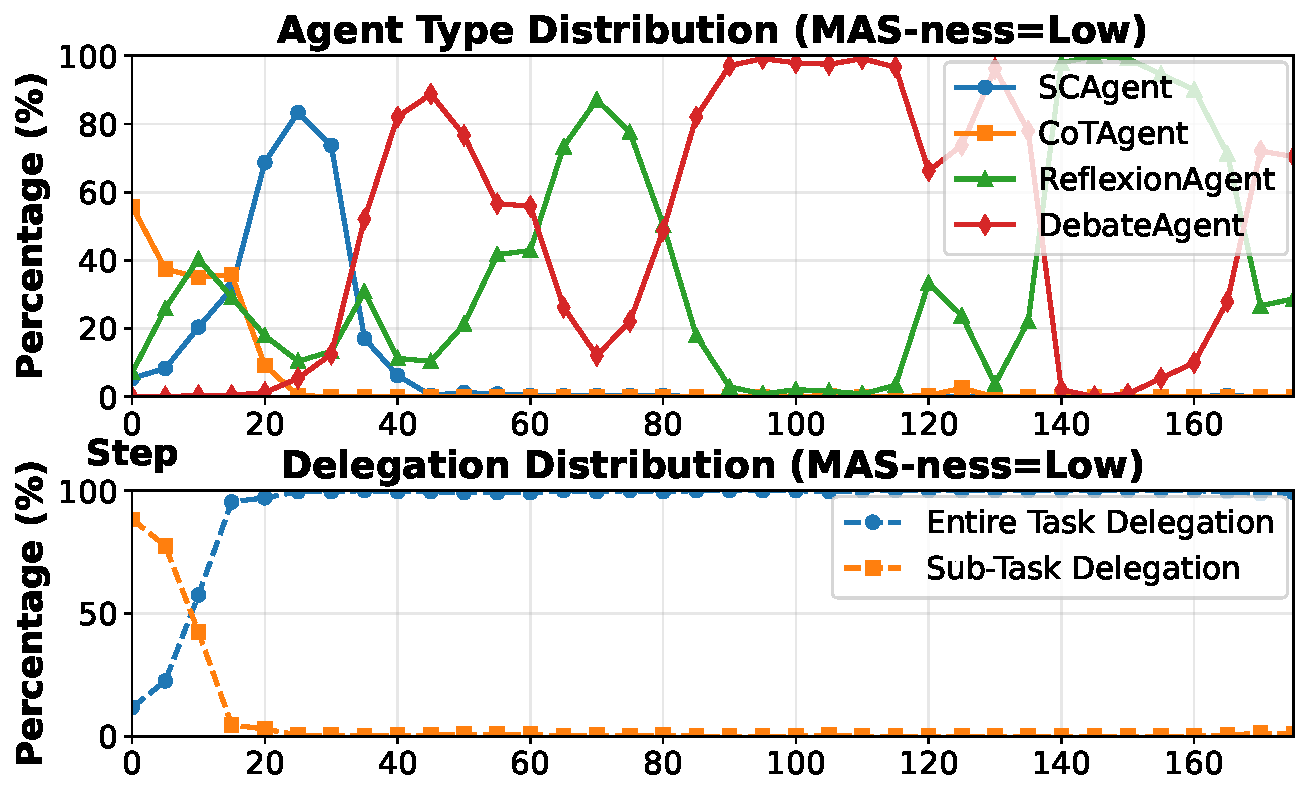
\includegraphics[width=0.5\columnwidth]{figs/7b_120b_aime24_low.pdf}
% \vspace{-1.5\baselineskip}
\captionof{figure}{\small 低 \masness 下的智能体统计（AIME24）。}
\label{fig:7b_120b_aime24_low}
\end{center}


\begin{figure*}[h]
\centering
% \vspace{-2\baselineskip}
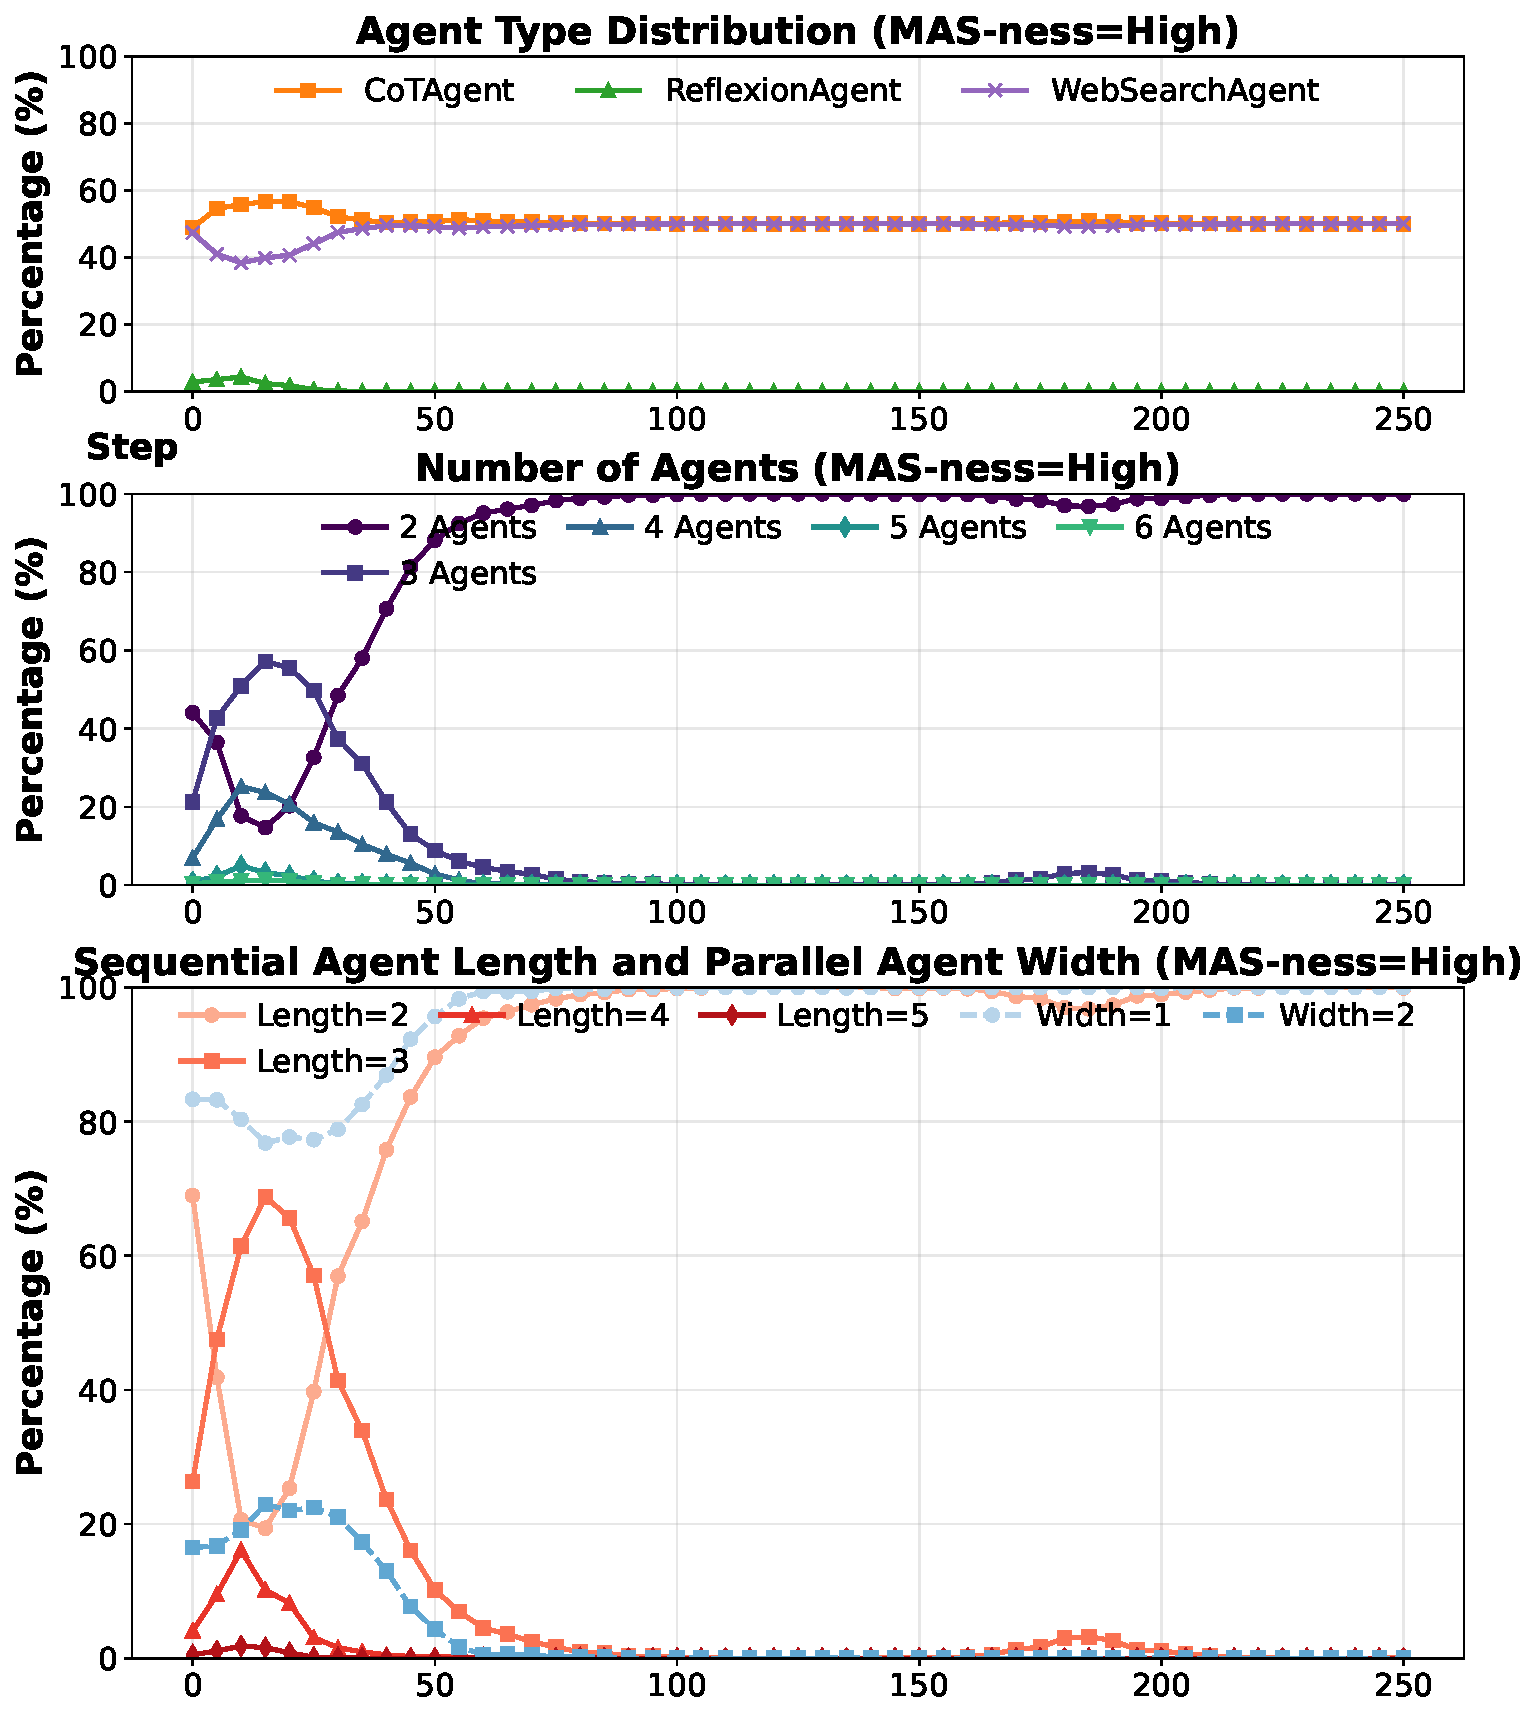
\includegraphics[width=0.5\columnwidth]{figs/7b_120b_hotpotqa_high.pdf}
% \vspace{-\baselineskip}
\captionof{figure}{\small 高 \masness 下的智能体统计（HotpotQA）。}
\label{fig:7b_120b_hotpotqa_high}
\end{figure*}

\begin{center}
% \vspace{-2\baselineskip}
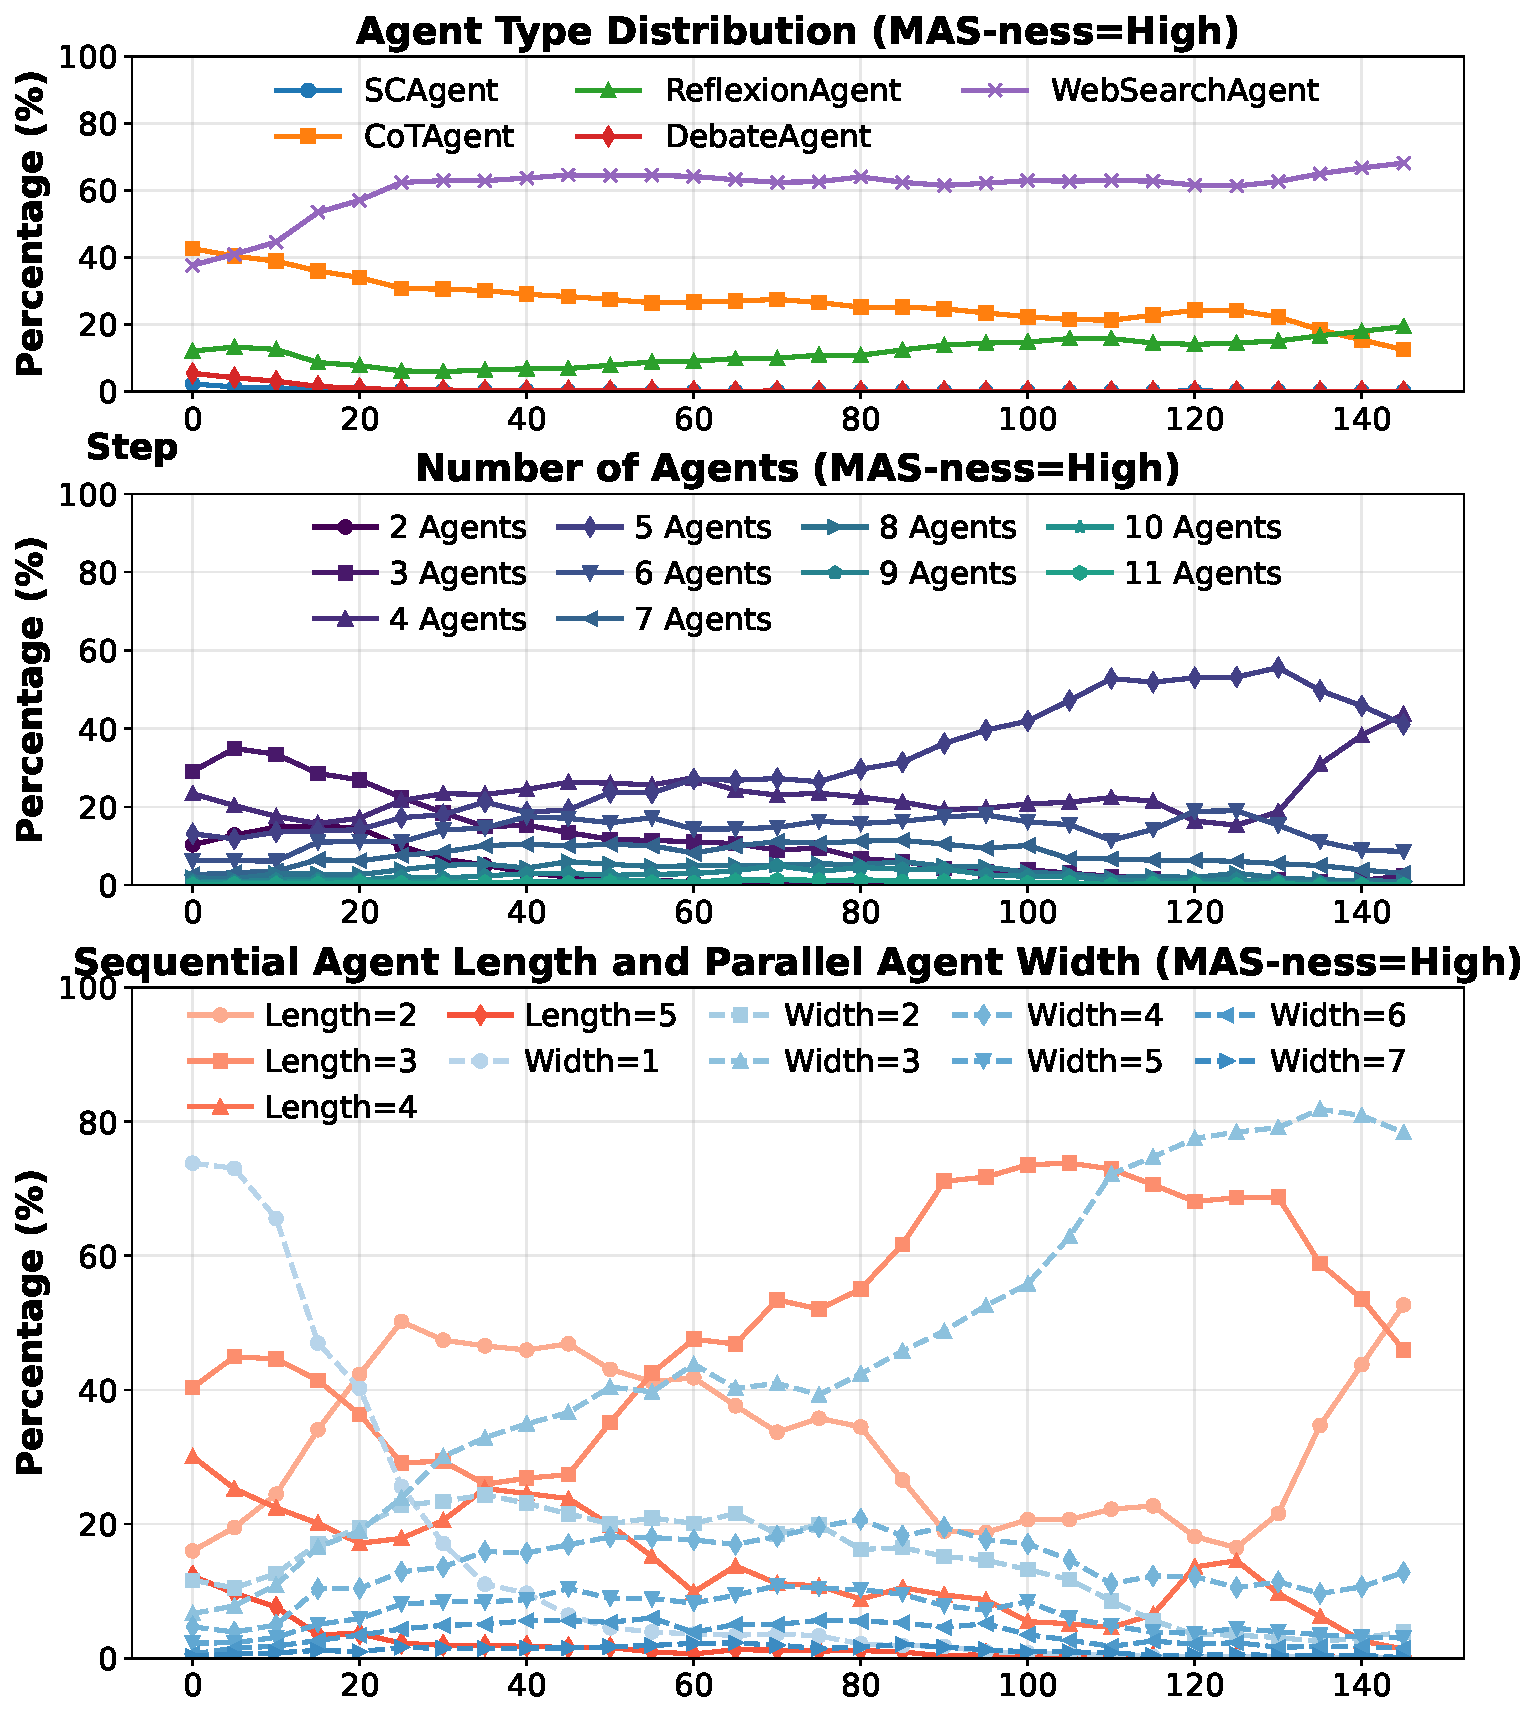
\includegraphics[width=0.5\columnwidth]{figs/7b_120b_browse_comp_plus_high.pdf}
\vspace{-0.5\baselineskip}
\captionof{figure}{\small 高 \masness 下的智能体统计（BrowseComp+）。}
\label{fig:7b_120b_browse_comp_plus_high}
\end{center}

% \zixuan{the others are more like generalization, no tracking during training}


\subsection{基准与生成的 MAS}
\label{ap:benchmark_generated_mas}

除\cref{sec:experiemnt}报告的结果外，我们还在\cref{fig:7b_120b_hotpotqa_high}中给出了 HotpotQA 的统计信息。
% \textbf{MAS patterns.}
% For AIME24, AIME25, and GPQA, the orchestrator effectively selects the best-performing sub-agent, which is typically the DebateAgent. This suggests that, for reasoning-intensive tasks with limited external information needs, selecting a strong reasoning sub-agent is sufficient.
对于 HotpotQA，尽管问题可能允许并行搜索，编排器往往只使用一个 \texttt{SearchAgent}（再加上最终的 \texttt{CoTAgent}，共两个智能体）。这说明这些问题相对简单，一次搜索便足以解决。

结合图~\ref{fig:7b_120b_aime24_low}中的 AIME 结果与图~\ref{fig:7b_120b_browse_comp_plus_high}中的 BrowseComp+ 结果，这些观察表明 \ourframework 能够动态适应给定任务：它会提出与底层子任务结构相符的 MAS 设计，并把执行委派给最有效的智能体配置。需要指出的是，由于底层 LLM 能力各异，生成的 MAS 设计不一定与底层任务结构完全一致（例如 HotpotQA）；这恰恰凸显了它相对于人工设计编排策略的优势。

% We note that this is expected as the orchestrator optimizes only for performance and does not explicitly consider cost or efficiency.

% For BrowseComp+, the orchestrator generates substantially more search agents. The typical pattern first retrieves all potentially required information through multiple search agents and then introduces an organization or aggregation agent to combine the retrieved results. This behavior is intuitive under a single-step reinforcement learning strategy, where collecting comprehensive evidence before aggregation can improve final-answer correctness.



% MAS Pattern: For AIME24, AIME25 and GPQA, orchestrator effectively select the good eprformaining sub-agent (typically DebateAgent). For HotpotQA, orchestrator decided to use only one search agent, while the question may have parallel searches. This indicates the question is relatively simple and one search is good enough (also our orchestrator only considers performance, not cost or efficiency). For BrowseComp+, much more search agents are createad. It typically first searches for all potential required information, and have an organizarion agent to aggregate all the searched results. (this makes intuitively sense for a single-step RL stategy)

% \zixuan{TODO Appendix: add more examples/statistics, e.g, how the 5 agents looks like, why they are good... so that we can discuss more here}


\subsection{成本比较}
\label{ap:cost_breakdown}



\cref{fig:parato_front}展示了成本-性能权衡，\cref{tab:cost_breakdown}则报告了 AIME24 与 GPQA 上相应的详细推理成本。整体式编排预计会比顺序式编排系统更高效，相较推理时编排方法的优势则更为明显。与这一直觉一致，按 LLM 调用次数、词元数量（包括提示词元和补全文本词元）与总成本计算，\ourframework 的效率提升均超过 \textbf{10$\times$}（成本基于撰写本文时 Together AI 的定价）。我们还观察到明显更快的实际运行时间。需要注意的是，实际运行时间不仅反映算法设计，也取决于实现细节；我们进行了大量优化（例如异步执行子智能体），并将向社区发布完整代码库。

% We note that in AIME24 and GPQA, which, as mentioned in \cref{sec:experiemnt}, mainly has the seqeuntail natural, SAS or simple standalone sub-agent can outperformes other automatic MAS design system as they are not in the regime of the edge of the sub-agent cometenece

% \zixuan{TODO: description: walltime is probably not very informative as it relates to implementaiton, async, etc., our implementaion optimize quite a bit on this.}


\begin{table}[h]
\centering
\small
\setlength{\tabcolsep}{6pt}
\renewcommand{\arraystretch}{1.15}
\begin{tabular}{lcccccccc}
\toprule
& \multicolumn{4}{c}{\textbf{AIME24}} & \multicolumn{4}{c}{\textbf{GPQA}} \\
\cmidrule(lr){2-5} \cmidrule(lr){6-9}
\textbf{方法}
& \textbf{调用}
& \textbf{词元（M）}
& \textbf{成本（\$）}
& \textbf{时间（ks）}
& \textbf{调用}
& \textbf{词元（M）}
& \textbf{成本（\$）}
& \textbf{时间（ks）} \\
\midrule
CoTAgent
& 30 & 0.05 & 0.03 & 0.38
& 198 & 0.16 & 0.06 & 1.18 \\
SCAgent
& 156 & 0.25 & 0.13 & 1.88
& 990 & 0.80 & 0.29 & 5.43 \\
DebateAgent
& 332 & 0.37 & 0.13 & 2.29
& 2178 & 2.04 & 0.55 & 7.65 \\
ReflexionAgent
& 112 & 0.14 & 0.06 & 0.67
& 518 & 0.44 & 0.13 & 2.50 \\
\midrule
MaAS
& 501 & 1.28 & 0.62 & 6.96
& 2936 & 7.52 & 3.11 & 39.52 \\
AFlow
& 1288 & 3.47 & 1.46 & 19.28
& 7404 & 12.38 & 4.52 & 56.94 \\
\midrule
MAS-GPT
& 228 & 0.74 & 0.37 & 5.47
& 1516 & 3.90 & 1.76 & 29.56 \\
ToolOrchestra
& 1319 & 3.77 & 1.76 & 31.35
& 7829 & 15.38 & 5.79 & 92.47 \\
\midrule
\textbf{\ourframework}
& \textbf{51} & \textbf{0.03} & \textbf{0.01} & \textbf{0.50}
& \textbf{261} & \textbf{0.22} & \textbf{0.07} & \textbf{0.46} \\
\bottomrule
\end{tabular}
\caption{AIME24 与 GPQA 上的推理时统计。词元数以百万（M）为单位，实际运行时间以千秒（ks）为单位。}
\label{tab:cost_breakdown}
\end{table}
